%%
%% Copyright 2007-2020 Elsevier Ltd
%%
%\documentclass[preprint,12pt]{elsarticle}
\documentclass[final,5p,times,twocolumn]{elsarticle}
\usepackage[utf8]{inputenc}
 \usepackage{amssymb}
 \usepackage{float}
 \usepackage{amsmath}
\usepackage{booktabs}
\usepackage{textcomp}
\usepackage{multirow}
\usepackage{siunitx}
\usepackage{xcolor}
\usepackage{pgfplots}
\usepgfplotslibrary{colormaps,groupplots,statistics}
\pgfplotsset{compat=1.18}
\usepackage{tikz}
\usetikzlibrary{shapes,arrows.meta,positioning,fit,backgrounds,calc}
\setlength{\marginparwidth}{2cm}
\usepackage{todonotes}
\graphicspath{{./}}
\definecolor{colorPure}{RGB}{180,180,180}
\definecolor{colorRAG}{RGB}{100,149,200}
\definecolor{colorHybrid}{RGB}{31,73,125}
 \journal{Decision Support Systems}
\begin{document}
\begin{frontmatter}
\title{Benchmarking LLM Integration Strategies for MCDA-Assisted Household Energy Decision Support}
\author{Ahaan Nigam}
\affiliation{organization={Downingtown East High School},
            city={Exton},
            state={PA},
            country={USA}}

\author{Dr. River Huang}
\affiliation{organization={Paul Scherrer Institut},
            city={Villigen},
            state={Aargau},
            country={Switzerland}}
\begin{abstract}
Households contribute 13\% of U.S.\ carbon emissions, yet most people rely on biased decision making rather than tailored choices. Multi-Attribute Value Theory (MAVT) offers a rigorous method of Multi-Criteria Decision Analysis (MCDA) to reduce emissions, but building MCDAs daily requires expertise that limits household adoption. This study evaluated whether LLMs can bridge that gap by comparing three architectures: Pure Prompting, Retrieval-Augmented Generation (RAG-Enhanced) Scoring, and a Hybrid of LLM parameter extraction with calculation. Ground truth calculators were built to benchmark MAVT scores across HVAC, appliance, and shower decisions. A total of 60 HVAC, 25 Appliance, and 15 Shower test scenarios were scored by each architecture, each with three alternatives scored on Environmental Impact, Energy Cost, Comfort, and Practicality with varying decision contexts. Hybrid achieved the strongest performance: Kendall's $\tau = 0.80$ and Spearman's $\rho = 0.82$, versus Pure Prompting's near-random $\tau = -0.06$ and $\rho = -0.055$. Top-1 accuracy reached 83\% for Hybrid versus 58\% for RAG-Enhanced and 30\% for Pure. Hybrid also achieved the lowest Mean Absolute Error (MAE) $= 0.69$ and Root Mean Squared Error (RMSE) $= 1.52$, fewest total tokens (98,016 vs.\ RAG-Enhanced's highest of 308,637), and lowest total latency (275.6s versus Pure's highest of 437.1s), despite higher per-call complexity. These results confirm that independent LLMs cannot be used to replicate MCDA creation, and that using LLMs to extract parameters for calculation is both the most accurate and most efficient path toward accessible household energy decision support.
\end{abstract}
\begin{keyword}
Large language models \sep Multi-criteria decision analysis \sep Multi-Attribute Value Theory \sep Household energy \sep Decision support systems \sep Retrieval-Augmented Generation \sep Sustainability
\end{keyword}
\end{frontmatter}

\section{Introduction}
\label{sec1}

The average U.S. household emits 8744 pounds of CO\textsubscript{2}e \cite{EPA2025} and uses 10,791 Kilowatt Hours of energy \cite{EIA2022} annually. Including transportation, food, etc., per capita, the numbers change to about 17.9 tons of CO2e \cite{CSS2024}, and 81767 Kilowatt Hours of energy annually \cite{EIA2022}. The average U.S. household can save \$200-\$400 annually by optimizing their house to ENERGY STAR recommendations \cite{DOE2025}.

\begin{figure}[H]
	\centering
	
\includegraphics[width=0.3\textwidth]{PAResidentialEmissions.png}
	\caption{Residential Emissions of the past 50 years (EIA, 2022)}
	\label{fig:intro-placeholder-1}
\end{figure}


Unfortunately, most Americans are not aware of the areas where they could be reducing their impact, which is why there is such a large amount of waste. This suggests a need for tools that combine optimization, behavioral insight, and decision support.

Multiple studies have shown that MCDAs, Life Cycle Assessments (LCA), and models for prediction such as Pareto Analysis have been effectively implemented to track and reduce environmental impact in larger sample sizes \cite{Collinge2014}. While engineering frameworks can potentially optimize decisions, producing them requires complexity and time: the Hilbert-Huang transform, among other conversion methods, are not rapid \cite{Cerneviciene2022}. In order to streamline the process, He Huang and his associates created a calculator that used multiple different accepted methods to get a reliable output \cite{HuangBurgherr2024}. The problem is, even with the simplicity of the calculator, some knowledge of MCDAs and creating a file to be utilized by the calculator is required - and educating each individual participant in our study would require extensive effort.


While the average U.S. household consumes 10,791 kWh annually, this consumption is not evenly distributed. Space heating accounts for approximately 43\% of residential energy use, followed by appliances (13\%), water heating (12\%), and air conditioning (8\%) (EIA, 2020). This distribution highlights key intervention points for emissions reduction. National reform of certain key household practices could result in a 123 million metric tonne (MtC) reduction in carbon per year as of 2005, when residential emissions accounted for 38\% of overall US CO2 emissions, or 626 MtC. Additionally, these changes would result in little to no reduction in satisfaction, a necessary factor in widespread implementation. Dietz et al. (2009) demonstrated that household-level behavioral changes, if widely adopted, could cut U.S. emissions by 123 MtC annually. However, concerns for behavioral plasticity-how likely people are to implement each action based on financial and social incentives-remain an important factor.



Figure 2 (Dietz et al., 2009) displays the behavioral plasticity, net carbon effect, and Reasonably Achievable Emission Reduction (RAER).
\begin{figure}[htbp]
	\centering
	
\includegraphics[width=0.5\textwidth]{LifestyleChangesEmissionImpact.png}
	\caption{Household behavior changes impact on emissions}
	\label{fig:intro-placeholder-2}
\end{figure}

A major challenge with implementing an MCDA-type framework is the extra work required from users; although the benefits may be clear, some groups may not desire a switch in their routine, and have to wait for and consult a generated framework constantly. The decisions that the frameworks would be used for, such as purchasing a specific product or adjusting the thermostat, are often made using heuristics.

Heuristics-quick decision making-are useful in everyday life, but under complex or high-stakes situations, they can lead to errors; multiple studies have found that under time pressure, people default to ``satisficing'' (choosing the first option that meets minimum criteria) or using dominant past behaviors, even if they're not ideal (Klapproth et al., 2008). Additionally, when these time constraints are combined with information overload, decision errors increase by approximately 20\% more errors in judgement (Hahn et al., 1992). Since energy-use decisions often occur in high-distraction environments, tools that rely on sustained attention or complex input formats may fail to influence user behavior effectively. Very limited empirical research has been conducted thus far on using decision frameworks (especially MCDAs) in residential sectors.

AI is increasingly being used to create decision frameworks such as MCDAs. It has shown promise in the Marketing and Medical industries. (Jackson et al., 2024; Huang \& Rust, 2020; Simon et al., 2024). Several studies have implemented frameworks, such as LCAs, MCDAs, MCDMs, Pareto Analysis, etc. successfully in environmental optimization decision making at a corporate or larger scale. AI's ability to manage large datasets suggests it could scale down to personal decision-making as well.

There is one substantial problem: constructing a framework typically requires extensive knowledge of MCDA construction methods (depending on the situation, certain ones often perform better than others), rubric design, and knowledge of the decision at hand. To remedy this, Huang and Burgherr (2024) created a calculator that assesses the situation and the criterion, and is able to evaluate the result. Although much more efficient than before, it still requires users
to understand how to diagnose a situation’s problems and be able to format them appropriately. As a result, they remain inaccessible to the average household.

Using an AI in conjunction with an MCDA analysis tool would help remedy this issue; it would allow a participant to describe their situation in normal English, convert it to a series of alternatives with weights, taking into account the local weather conditions, electricity rates, etc. through APIs. 

AI has been used to create MCDAs before by Igor Svoboda and Dmytro Lande (2024) in a study on cybersecurity analysis. They found that GPT-4 had a consistency ratio well below the accepted ratio of 0.1, which means that the decision outputs were coherent. They also tested a number of other AIs, such as GPT-3, which was found to be unreliable. This study tested and proved that AI models are reliable enough to use with decision frameworks, helping reinforce the plausibility of my research. 

Modern systems also have a general knowledge of the energy use and carbon footprint of most products, among other metrics. AI has the ability to deduct these statistics from its own information, and also search the internet for useful information. However, AI has not been rigorously tested for individual-level decisions using longitudinal performance data. 

Additionally, AI systems tend to create potential biases by assuming pieces of knowledge, such as assuming the same climate patterns or energy sources apply across all locations.(Galaz et al., 2021; Nishant et al., 2020).

Thus, while AI systems should have a decent capability to understand contexts and predict scores based on knowledge, having a RAG database and/or a calculator to actually help back up their reasoning would likely help prevent multiple biases. This framework has not been tested in a real-world individual context, so empirical data is limited. This study aims to contribute early insights into how such tools, and which methods, are best to deploy widely.

The convergence of these three research areas (household emissions, behavioral barriers, and AI-assisted decision frameworks) point to a clear opportunity. MAVT offers a mathematically sound way to compare tradeoffs between aspects of practicality, comfort, cost, and the environment. The natural language interface offered by LLMs eliminates the technical obstacle to utilizing these frameworks. The remaining questions are which integration architecture best maintains the mathematical rigor that initially makes MCDA valuable and whether LLMs can score criteria accurately enough to be trusted. Without addressing this, any tool based on these principles runs the risk of making confident but inaccurate recommendations, which could be worse than having no tool at all.

This study directly addresses that question by comparing three architectures with varying levels of assistance against calculations made with further specified information. We focused on three different contexts-Pure Prompting, RAG-Enhanced, and Hybrid parameter extraction-specifically for household energy decision-making by testing across [NUMBER] scenarios, determining which method best replicates an actual expert's MCDA scoring.

\section{Methodology}
\label{sec2}

\subsection{Decision Types and Scenario Corpus}

Three specific decision types were chosen due to their high plasticity and RAER, as well as being timely, everyday decisions that may change constantly. These were HVAC-related decisions, which are about temperature control, Appliance-related decisions, which are about the time of day (TOD) to use appliances, and Shower-related decisions, which are about how long to shower for. Each of the 3 architectures were tested on a 263-scenario corpus that was divided into 128 HVAC, 80 Appliance, and 55 Shower decisions. They were compared to a calculated, decision-type specific dataset from a calculator. This calculator also ran on an additional 77 RAG scenarios, split into 37 HVAC, 30 Appliance, and 10 Shower for a retrieval augmented generation (RAG) database.

The HVAC decision type was the most complex. The table below details the parameters given to architectures vs. calculators. 

\begin{table}[htbp]
\centering
\small
\caption{HVAC parameters: Architectures vs. calculator}
\label{table:hvac_parameters}
\begin{tabular}{@{} l c c @{}}
\toprule
\textbf{Parameter} & \textbf{LLMs} & \textbf{Calc.} \\
\midrule
Location & \checkmark & --- \\
Outdoor Temp & \checkmark & \checkmark \\
Home Size (sqft) & \checkmark & \checkmark \\
Insulation & \checkmark & --- \\
R-Value & --- & \checkmark \\
Household Size & \checkmark & \checkmark \\
Housing Type & \checkmark & \checkmark \\
House Age & \checkmark & \checkmark \\
Utility Budget & \checkmark & --- \\
SEER Rating & --- & \checkmark \\
Occupancy Context & --- & \checkmark \\
Indoor Temp (from alternative) & --- & \checkmark \\
\bottomrule
\end{tabular}
\end{table}

% Reasoning placeholder for HVAC parameters
[REASONING PARAGRAPHS FOR HVAC PARAMETERS]


% Appliance parameters table
\begin{table}[htbp]
\centering
\small
\caption{Appliance parameters: Architectures vs. calculator}
\label{table:appliance_parameters}
\begin{tabular}{@{} l c c @{} }
\toprule
\textbf{Parameter} & \textbf{LLMs} & \textbf{Calc.} \\
\midrule
Appliance Type & \checkmark & \checkmark \\
kWh per Cycle & --- & \checkmark \\
Cycle Duration (min) & \checkmark & \checkmark \\
Preferred Run Time & \checkmark & --- \\
TOU Period & \checkmark & \checkmark \\
Baseline Time & \checkmark & --- \\
Efficiency Rating & \checkmark & \checkmark \\
Household Size & \checkmark & \checkmark \\
Utility Rate & \checkmark & \checkmark \\
Monthly Cycles Assumption & --- & \checkmark \\
Utility Budget & \checkmark & --- \\
\bottomrule
\end{tabular}
\end{table}

[REASONING PARAGRAPHS FOR APPLIANCE PARAMETERS]

% Shower parameters table
\begin{table}[htbp]
\centering
\small
\caption{Shower parameters: Architectures vs. calculator}
\label{table:shower_parameters}
\begin{tabular}{@{} l c c @{} }
\toprule
\textbf{Parameter} & \textbf{LLMs} & \textbf{Calc.} \\
\midrule
Location & \checkmark & --- \\
Outdoor Temp & \checkmark & \checkmark \\
Inlet Water Temp & --- & \checkmark \\
Heater Setpoint & \checkmark & \checkmark \\
Flow Rate (GPM) & --- & \checkmark \\
Duration (min) & \checkmark & \checkmark \\
Household Size & \checkmark & \checkmark \\
Water Heater Type & \checkmark & \checkmark \\
Tank Size & --- & \checkmark \\
Utility Budget & \checkmark & --- \\
Occupancy Frequency & \checkmark & --- \\
\bottomrule
\end{tabular}
\end{table}

[REASONING PARAGRAPHS FOR SHOWER PARAMETERS]




\subsection{MAVT Framework Design ALL OF THESE PARAS NEED MORE SPECIFICS}
Residential emissions represent one of the most controllable contributors to national carbon output. Space heating accounts for approximately 43\% of residential energy use, followed by appliances (13\%), water heating (12\%), and air conditioning (8\%) (EIA, 2020). This distribution highlights key intervention points for emissions reduction. Dietz et al. (2009) demonstrated that household-level behavioral changes, if widely adopted, could cut U.S. emissions by 123 MtC annually. 

[ENVIRONMETNAL WEIGHTING REASONING]

The biggest factor on consumer behavior was the cost savings, although this decreased in influence if the consumer cared less about future savings (Newell \& Siikamaki). In fact, a study on consumers estimating the energy usage of different appliances found that they undervalued "energy use and savings by a factor of 2.8 on average, with small overestimates for low-energy activities and large underestimates for high-energy activities" (Attari et al.). In another study of the effectiveness of energy labels in providing information that influenced customer decisions found that once the statistics on cost savings were unclear (e.g. the label did not state any kind of measurable number for energy reduction), the impact of all information dropped significantly (Allcott et al., Davis \& Metcalf). Thus, it is important for the predicted energy use to be shown and for the resulting cost savings to be heavily emphasized. [ADD MORE]

[Energy Cost WEIGHTING REASONING]

COMFORT PARA + REASONING

A major challenge with implementing MCDAs, or even a tool to help make decisions, is the extra work required from users; although the benefits may be clear, some groups may not desire a switch in their routine. (Zakay \& Ariely)(Leclerc et al.) 

The decisions that the frameworks would be used for, such as purchasing a specific product or adjusting the thermostat, are often made using heuristics. Choosing to do something using heuristics will almost always be easier than using a model. Thus, proving the practicality of the chosen decision while ensuring that it falls within budget and system limits ensures that the user has more reason to trust the tool.

\begin{table}[htbp]
\centering
\small
\caption{Reference ranges (5th--95th percentiles) by Criterion}
\label{table:reference_ranges}
\begin{tabular}{@{}lccc@{}}
\toprule
\textbf{Criterion} & \textbf{HVAC} & \textbf{Appliance} & \textbf{Shower} \\
\midrule
Energy Cost (\$) & 0.47 – 3.31 & 0.017 – 1.12 & 0.15 – 1.50 \\
Environmental Impact & 2.42 – 18.14 & 0.244 – 3.644 & 7.5 – 75.0 \\
Comfort & 0.0 – 10.0 & 0.0 – 10.0 & 0.0 – 10.0 \\
Practicality & 0.5 – 10.0 & 0.5 – 10.0 & 0.5 – 10.0 \\
\bottomrule
\end{tabular}
\end{table}

The above reference ranges were derived for the MAVT normalization.
The reference ranges in Table~\ref{table:reference_ranges} are grounded in the ground-truth calculators and reflect the 5th--95th percentiles of the scenario distributions rather than extreme theoretical limits, so that normalization preserves meaningful spread across typical residential alternatives. For HVAC energy cost, the percentile envelope is anchored to empirical efficiency and degradation studies (efficient systems: \cite{huyen2019,kim2024,cetin2015}; degraded systems: \cite{alves2016,krarti2020}) and evaluated at a standardized 8-hour window with Pennsylvania's residential electricity rate. The HVAC environmental bounds are derived from the same kWh envelope mapped through PJM marginal emissions factors, maintaining a physically consistent link between cost and emissions while avoiding over-weighting rare tail cases.

For appliances, the minimum cost bound combines a 5th-percentile per-cycle energy use for efficient HE washers with the lowest off-peak utility rate, while the maximum bound expands ENERGY STAR's upper kWh/cycle benchmark to cover older resistance dryers and pairs it with the highest peak rate; the environmental range applies the same kWh envelope to PJM marginal emissions factors. Shower cost bounds are computed from a realistic low-flow, short-duration summer case versus a higher-flow, long-duration winter case, with inlet temperature modeled from NREL data and duration distributions drawn from REU2016 and the Harris Poll \cite{reu2016,harrispoll2024,hendron2008}. Shower environmental impact is defined as water volume (gallons), using WaterSense flow-rate percentiles and 5--15 minute duration ranges, while comfort is standardized to 0--10 and practicality uses a 0.5 floor to avoid collapsing the value function at the lower bound.

The HVAC energy-cost range reflects the 5th--95th percentile of the scenario cost distribution under an 8-hour run window at \$0.19/kWh, with endpoints anchored to residential HVAC efficiency and degradation studies (efficient systems: \cite{huyen2019,kim2024,cetin2015}; degraded systems: \cite{alves2016,krarti2020}). The HVAC environmental range is derived from this same kWh envelope, mapped through PJM marginal emissions factors for off-peak and peak generation; the intent is to preserve a consistent physical linkage between cost and emissions while keeping the normalization centered on typical residential alternatives.

For appliances, the cost bounds combine a 5th-percentile per-cycle energy use (0.25 kWh for efficient HE washers) with the lowest off-peak rate and a 95th-percentile upper envelope (energy use expanded from ENERGY STAR's 2.82 kWh/cycle to 3.5 kWh/cycle to cover older resistance dryers) with the highest PECO peak rate; the environmental bounds apply the same kWh envelope to PJM marginal emissions factors. Shower energy-cost bounds are based on flow-rate and duration extremes under realistic seasonal inlet temperatures (low-flow, short summer case vs. higher-flow, long winter case), drawing on REU2016 shower-duration data, Harris Poll prevalence of long showers, and NREL inlet-temperature modeling (\cite{reu2016,harrispoll2024,hendron2008}). For showers, environmental impact is defined as water volume (gallons), using WaterSense 5th--95th percentile flow rates and 5--15 minute duration ranges; comfort is standardized to a 0--10 scale, and practicality uses a 0.5 floor to avoid collapsing the value function at the lower bound.
% Reasoning placeholder for HVAC parameters
[ATTRIBUTE SOURCES TO EACH VALUE AND JUSTIFY]
\subsection{Ground Truth Calculators}



- Describe what each calculator computes: energy cost in \$, comfort, and practicality are
    consistent across all three decision types.
- Environmental impact is measured in lbs CO$_2$ for HVAC and Appliance,
    computed from kWh consumption using Pennsylvania PJM marginal emissions
    factors (peak: 1.041 lbs CO$_2$/kWh; off-peak: 0.976 lbs CO$_2$/kWh).
    For Shower, environmental impact uses water consumption (gallons) as a
    proxy, since the dominant environmental burden of shower decisions is
    hot water volume rather than grid-electricity emissions; full derivation
    in Appendix A.3.
- Cite sources for each formula (ASHRAE, Domanski, NREL, EPA eGRID PJM,
    PECO TOU, REU2016 for shower frequency)
- Full derivations in Appendix A

2.4 Architecture Implementations

- 2.4.1 Pure Prompting
- 2.4.2 RAG-Enhanced (ChromaDB, sentence-transformers/all-MiniLM-L6-v2, k=3)
- 2.4.3 Hybrid
- LLM: Mistral Small 3.2 24B, T=0.3, OpenRouter
- API call structure: 3 calls/scenario (Pure, RAG) vs.\ 1 call/scenario (Hybrid)

2.5 Evaluation Metrics

- Accuracy: Kendall's $\tau$, Spearman's $\rho$, Top-1, Top-2, MAE, RMSE
- Efficiency: total tokens, total latency

Appendix A --- Ground Truth Calculator Formulas

A.1 HVAC Calculator (cooling load, heating load, SEER degradation, TOU)
A.2 Appliance Calculator (kWh/cycle, TOU pricing tiers, budget penalty)
A.3 Shower Calculator (water heating energy, GPM $\times$ duration; environmental
    criterion = water consumption in gallons, not CO$_2$)

Appendix B --- Reference Ranges and Constants

- Table of all 5th--95th percentile reference ranges by decision type and criterion
- PA constants: electricity rate \$0.19/kWh; PJM marginal emissions factors
    (peak: 1.041 lbs CO$_2$/kWh, off-peak: 0.976 lbs CO$_2$/kWh); TOU multipliers
- Energy cost reference ranges:
    HVAC \$0.47--\$3.31; Appliance \$0.017--\$1.12; Shower \$0.15--\$1.50
- Environmental reference ranges (lbs CO$_2$):
    HVAC 1.60--11.25; Appliance 0.09--3.83
- Environmental reference range (gallons):
    Shower: see Appendix A.3

\section{Results}
\label{sec3}

3.1 Overall Ranking Accuracy

- Summary table: $\tau$, $\rho$, Top-1, Top-2 for all three architectures
    (Hybrid: $\tau=0.80$, $\rho=0.82$, Top-1=83\%, Top-2=97\%)
    (RAG: $\tau=0.43$, Top-1=58\%, Top-2=89\%)
    (Pure: $\tau=-0.06$, Top-1=30\%, Top-2=62\%)
- Statement that Hybrid dominates on all ranking metrics; Pure is near-random
- Note that RAG shows meaningful improvement over Pure,
    confirming retrieval context adds signal but not sufficient alone

3.2 Criterion-Level Error (MAE and RMSE)

- Table: MAE and RMSE per criterion $\times$ architecture
- Call out anomalies:
        - Hybrid HVAC Comfort + Practicality MAE = 0.0
            (deterministic from occupancy context --- fully correct)
        - RAG Appliance Comfort MAE = 3.88 (worst in dataset ---
            subjective criterion with no formula anchor)
        - Pure Shower Environmental MAE = 4.04 (second worst ---
            no retrieval, no calculator; environmental criterion for Shower
            is water consumption in gallons, a behavioral proxy that
            LLMs systematically misestimate without GPM and duration inputs)
- Note that quantitative criteria (Energy Cost, Environmental)
    show the largest gap between Hybrid and the other two

3.3 Performance by Decision Type

- Table or grouped bar chart: $\tau$ by architecture $\times$ decision type
    (Hybrid HVAC $\tau=0.90$ vs.\ Appliance $\tau=0.68$ vs.\ Shower $\tau=0.60$)
    (RAG HVAC Top-1=63\% as best RAG result)
    (Pure Appliance gap vs.\ Hybrid is largest --- MAE 3.31 vs.\ 0.97)
- Explanation that HVAC is the most structured decision type,
    benefiting both RAG (clean energy tradeoffs map to database)
    and Hybrid (deterministic comfort/practicality extraction)
- Appliance and shower performance gaps explained by absence
    of a structural anchor equivalent to occupancy context

3.4 Token Usage and Latency

- Table: total tokens + total latency per architecture
    (Hybrid: 98,016 tokens, 275.6s)
    (Pure: 124,709 tokens, 437.1s)
    (RAG: 308,637 tokens, 480.8s)
- Note the counterintuitive result: Hybrid is token-cheapest
    despite structured output requirements --- 100 calls vs.\ 300
    for Pure/RAG more than compensates for per-call complexity
- RAG is most token-expensive due to retrieval context
    appended to every prompt
- Hybrid is simultaneously the fastest, most accurate,
    and most token-efficient architecture

\section{Discussion}
\label{sec4}

4.1 Why Hybrid Works: Architecture Separates NL from Math

- Core argument: LLMs are strong at extracting structured
    parameters from natural language; they are not reliable
    at physics-based quantitative scoring end-to-end
- Hybrid's design exploits the LLM's actual strength
    (extraction) while offloading its weakness (formula math)
    to the calculator
- Single API call per scenario is both architecturally simpler
    and empirically faster --- not a bias but a design advantage
- Svoboda \& Lande (2024) showed LLMs can produce coherent MCDA
    structures --- this study extends that: coherent structure is
    not the same as accurate quantitative scoring

4.2 Why Pure Prompting Fails

- Near-random $\tau = -0.06$ confirms LLMs cannot self-generate
    physics-based MAVT scores from scenario text alone
- No grounding in reference ranges $\to$ uncalibrated 0--10 scores
    that are internally consistent per call but not comparable
    across alternatives or criteria
- Risk point: a tool built on Pure Prompting would produce
    confident but wrong recommendations --- potentially worse than
    no tool at all (cite back to Introduction's framing)

4.3 Why RAG Is Intermediate --- and Where It Helps

- Retrieval adds meaningful signal for structured decision types
    (HVAC: $\tau$ jumps from near-random to 0.52 for RAG)
- Retrieval cannot substitute formula-based reasoning for
    criteria that require exact TOU rate math or GPM calculations
- RAG's Top-2 = 89\% suggests it could be a useful low-cost
    fallback where getting the top-2 correct is acceptable and
    building a full calculator is not feasible
- Token cost (308,637) is the main practical barrier for RAG

- Entropy and implied regression both support an environmental weight $\geq 0.35$.
- MEREC's lower environmental estimate reflects within-scenario correlation with energy cost rather than reduced normative importance \cite{Keshavarz-Ghorabaee2021}.
- The inconsistency of practicality weights across methods is attributed to deterministic scores in the HVAC calculator (56\% zero-variance scenarios), which artificially inflates MEREC removal effects and suppresses implied regression coefficients.

4.4 Efficiency as a Practical Constraint

- Real household decision support requires low latency ---
    Hybrid's 275.6s across 100 scenarios scales to $\sim$2.8s/decision
- Token efficiency directly maps to API cost --- Hybrid is the
    only architecture viable at scale without significant cost
- Tradeoff: Hybrid requires upfront investment to build the
    physics-based calculators; RAG does not

4.5 Limitations

- Single LLM (Mistral Small 3.2 24B): unknown if Hybrid
    advantage holds for stronger models or closes for weaker ones
- Single region (Pennsylvania): PJM marginal emissions factors
    (peak: 1.041, off-peak: 0.976 lbs CO$_2$/kWh) and PPL TOU
    rate structure --- results may not generalize to high-renewables
    grids where environmental score compression changes which
    architecture performs best
- Shower environmental criterion uses water consumption (gallons)
    as a proxy rather than CO$_2$ emissions; this makes the
    environmental dimension semantically heterogeneous across decision
    types. The ranking logic and MAVT structure are unaffected,
    but cross-decision-type comparisons of environmental MAE should
    be interpreted with this proxy distinction in mind
- Researcher designed both ground truth and Hybrid calculator ---
    this is the most critical validity threat; Hybrid's advantage
    may reflect design alignment rather than architecture
    superiority (must be foregrounded, not buried)
- No statistical significance testing on $\tau$ differences between
    architectures --- genuine gap, not currently quantifiable
    as statistically significant
- Temperature fixed at 0.3 with single run per scenario ---
    no variance measurement across runs

\subsection{Limitations and Future Work}

4.6 Future Work

- Scenario-type-specific extraction prompts for Hybrid to
    address appliance/shower performance gap ($\tau=0.68$/$0.60$ vs.\
    HVAC $\tau=0.90$)
- Multi-region generalization using all EPA eGRID subregions
    + EIA real-time utility rate API
- Multi-model benchmarking: the same 100 scenarios are currently
    being benchmarked against Mistral Small 3.2 24B, Qwen 2.5 72B,
    Claude Sonnet 4, and Gemini 2.5 Pro via OpenRouter to isolate
    whether the architecture advantage holds across model classes and
    sizes; results are in preparation
- Real-world deployment study: mobile interface for PA
    households, longitudinal tracking of actual decisions
    vs.\ tool recommendations
- Standardized shower environmental criterion: replacing the
    water-consumption proxy with a lifecycle CO$_2$ factor (e.g.,
    water heating emissions per gallon) would enable consistent
    cross-decision-type environmental comparisons

\section{Conclusion}
\label{sec5}

- Restate research question: which LLM integration architecture
    most accurately replicates physics-based MAVT ground truth
    for household energy decisions?
- Direct answer: Hybrid ($\tau=0.80$, Top-1=83\%, MAE=0.69)
    outperforms RAG ($\tau=0.43$, Top-1=58\%) and Pure ($\tau=-0.06$, Top-1=30\%)
    on every accuracy and efficiency metric simultaneously
- Core finding: LLMs used end-to-end cannot replicate MCDA
    scoring; LLMs used for parameter extraction can
- Efficiency finding: Hybrid is simultaneously the most accurate
    and least resource-intensive architecture --- the expected
    token/efficiency tradeoff did not materialize
- Practical implication: the architecture that requires the most
    upfront research investment (building the physics calculators)
    is the only one suitable for a real household decision tool ---
    but once built, it is fast and cheap to run per decision
- Broader significance: this study provides the first empirical
    comparison of three LLM-MCDA integration strategies for
    individual household energy decisions, filling the gap between
    organizational-scale MCDA literature and routine household choice
- Call to action: the results support investment in LLM-assisted
    MCDA tools as a pathway to closing the intention-behavior gap
    in household sustainability decisions --- but only when grounded
    in deterministic calculation

\clearpage
\bibliographystyle{elsarticle-num}
\bibliography{cas-refs}

%% =====================================================================
%% ITEM 1 -- Notation Table
%% =====================================================================
\begin{table}[t]
\small
\centering
\renewcommand{\arraystretch}{1.15}
\begin{tabular}{ll}
\toprule
Symbol & Definition \\
\midrule
$\tau$ & Kendall's rank correlation coefficient \\
$\rho$ & Spearman's rank correlation coefficient \\
$w_i$ & weight of criterion $i$ ($i=1\ldots4$), summing to 1 \\
$v_i(x)$ & value function score for criterion $i$ at raw value $x$, range $[0,10]$ \\
$\alpha$ & shape parameter for logarithmic value functions \\
$s_j$ & MAVT weighted sum score for alternative $j$ \\
$\text{MAE}$ & Mean Absolute Error on MAVT score (0--10 scale) \\
$\text{RMSE}$ & Root Mean Squared Error on MAVT score (0--10 scale) \\
$n$ & number of test scenarios evaluated \\
$k$ & number of retrieved chunks per query in RAG ($k=3$) \\
\bottomrule
\end{tabular}
\renewcommand{\arraystretch}{1.0}
\caption{Notation used throughout this paper.}
\label{tab:item1}
\end{table}

%% =====================================================================
%% ITEM 2 -- MAVT Equations Block
%% =====================================================================
\begin{equation}
\label{eq:mavt_sum}
s_j = \sum_{i=1}^{4} w_i \cdot v_i(x_{ij})
\end{equation}

\begin{equation}
\label{eq:linear_vf}
v_i(x) = \frac{x - x_{\min}}{x_{\max} - x_{\min}} \times 10
\end{equation}

\begin{equation}
\label{eq:log_vf}
v_i(x) = \frac{\ln\!\left(1 + \alpha \cdot \frac{x - x_{\min}}{x_{\max} - x_{\min}}\right)}{\ln(1 + \alpha)} \times 10
\end{equation}

%% =====================================================================
%% ITEM 3 -- MAVT Framework Specification Table
%% =====================================================================
\begin{table}[t]
\small
\centering
\renewcommand{\arraystretch}{1.15}
\begin{tabular}{lllll}
\toprule
Criterion & Weight (\%) & Value Function & $\alpha$ & Direction \\
\midrule
Environmental Impact & 35 & Linear & \textemdash & Lower raw = better \\
Energy Cost & 30 & Linear & \textemdash & Lower raw = better \\
Comfort & 20 & Logarithmic & 1.5 & Higher raw = better \\
Practicality & 15 & Logarithmic & 1.2 & Higher raw = better \\
\bottomrule
\end{tabular}
\renewcommand{\arraystretch}{1.0}
\caption{MAVT criterion specification. Weights sum to 100\% and are held constant across all architectures and the ground truth calculator.}
\label{tab:item3}
\end{table}

%% =====================================================================
%% ITEM 4 -- Scenario Corpus and Parameter Asymmetry Table
%% =====================================================================
\begin{table*}[t]
\footnotesize
\centering
\begin{minipage}[t]{0.34\textwidth}
\centering
\renewcommand{\arraystretch}{1.15}
\begin{tabular}{lccc}
\toprule
Decision Type & Test Set ($n$) & RAG Set ($n$) & Total ($n$) \\
\midrule
HVAC & 60 & 25 & 85 \\
Appliance & 25 & 20 & 45 \\
Shower & 15 & 5 & 20 \\
\midrule
Total & 100 & 50 & 150 \\
\bottomrule
\end{tabular}
\renewcommand{\arraystretch}{1.0}
\end{minipage}
\hspace{2em}
\begin{minipage}[t]{0.60\textwidth}
\centering
\renewcommand{\arraystretch}{1.15}
\begin{tabular}{lll}
\toprule
Decision Type & GT Calculator Receives & Withheld / Generalized for AI \\
\midrule
HVAC & \parbox[t]{0.26\textwidth}{R-value, SEER, HVAC age, sq.\ ft., insulation, occupancy context} & \parbox[t]{0.26\textwidth}{R-value, HVAC age, SEER, occupancy context (insulation $\rightarrow$ good/avg/poor)} \\
Appliance & \parbox[t]{0.26\textwidth}{kWh/cycle, peak rate, off-peak rate, baseline time, appliance type} & \parbox[t]{0.26\textwidth}{All five: type, rates, kWh/cycle, baseline time} \\
Shower & \parbox[t]{0.26\textwidth}{Tank size, water heater temp, GPM} & \parbox[t]{0.26\textwidth}{Tank size, water heater temp} \\
\bottomrule
\end{tabular}
\renewcommand{\arraystretch}{1.0}
\end{minipage}
\caption{Left: scenario distribution. Right: parameters available to the ground truth calculator but withheld or generalized for AI input, by decision type.}
\label{tab:item4}
\end{table*}

%% =====================================================================
%% ITEM 5 -- Main Performance Summary Table
%% =====================================================================
\begin{table*}[t]
\footnotesize
\centering
\renewcommand{\arraystretch}{1.15}
\begin{tabular}{lccc}
\toprule
Metric & Pure Prompting & RAG-Enhanced & Hybrid \\
\midrule
\multicolumn{4}{l}{\textbf{Ranking Accuracy}} \\
Kendall's $\tau$ & -0.06 & 0.43 & \textbf{0.80} \\
Spearman's $\rho$ & -0.055 & 0.49 & \textbf{0.82} \\
Top-1 Accuracy (\%) & 30.00\% & 58.00\% & \textbf{83.00\%} \\
Top-2 Accuracy (\%) & 62.00\% & 89.00\% & \textbf{97.00\%} \\
\midrule
\multicolumn{4}{l}{\textbf{Score Error}} \\
Overall MAE & 2.52 & 1.61 & \textbf{0.69} \\
Overall RMSE & 3.07 & 2.40 & \textbf{1.52} \\
\bottomrule
\end{tabular}
\renewcommand{\arraystretch}{1.0}
\\[2pt]
{\small Scores on 0--10 MAVT scale. $n = 100$ scenarios.}
\caption{Overall performance comparison across all 100 test scenarios. Best value per metric in bold.}
\label{tab:item5}
\end{table*}

%% =====================================================================
%% ITEM 6 -- Criterion-Level MAE Table
%% =====================================================================
\begin{table}[t]
\small
\centering
\renewcommand{\arraystretch}{1.15}
\begin{tabular}{lccc}
\toprule
Criterion & Pure Prompting & RAG-Enhanced & Hybrid \\
\midrule
Energy Cost & 2.60 & 1.60 & \textbf{0.96} \\
Environmental Impact & 2.80 & 1.59 & \textbf{1.02} \\
Comfort & 2.51 & 1.97 & \textbf{0.32} \\
Practicality & 2.16 & 1.29 & \textbf{0.43} \\
\midrule
Overall & 2.52 & 1.61 & \textbf{0.69} \\
\bottomrule
\end{tabular}
\renewcommand{\arraystretch}{1.0}
\\[2pt]
{\small $^\dagger$Hybrid HVAC Comfort MAE = 0.00 and Practicality MAE = 0.00 (fully deterministic); reported separately in Table~\ref{tab:item7}. Environmental MAE for Shower reflects water-consumption proxy (gallons), not lbs CO$_2$; see Section 2.3.}
\caption{MAE per criterion by architecture (Overall, $n=100$, score 0--10). Best per criterion in bold.}
\label{tab:item6}
\end{table}

%% =====================================================================
%% ITEM 7 -- Per-Decision-Type Full Breakdown Table
%% =====================================================================
\begin{table*}[t]
\footnotesize
\centering
\renewcommand{\arraystretch}{1.15}
\begin{tabular}{lccccccccc}
\toprule
 & \multicolumn{3}{c}{Pure Prompting} & \multicolumn{3}{c}{RAG-Enhanced} & \multicolumn{3}{c}{Hybrid} \\
\cmidrule(lr){2-4}\cmidrule(lr){5-7}\cmidrule(lr){8-10}
Decision Type & $\tau$ & Top-1 (\%) & Top-2 (\%) & $\tau$ & Top-1 (\%) & Top-2 (\%) & $\tau$ & Top-1 (\%) & Top-2 (\%) \\
\midrule
HVAC ($n=60$) & -0.11 & 25.00\% & 56.67\% & 0.52 & 63.33\% & 93.33\% & \textbf{0.90} & \textbf{91.67\%} & 100.00\% \\
Appliance ($n=25$) & 0.09 & 40.00\% & 72.00\% & 0.41 & 56.00\% & 88.00\% & \textbf{0.68} & \textbf{72.00\%} & 92.00\% \\
Shower ($n=15$) & -0.11 & 33.33\% & 66.67\% & 0.11 & 40.00\% & 73.33\% & \textbf{0.60} & \textbf{66.67\%} & 93.33\% \\
\midrule
Overall ($n=100$) & -0.06 & 30.00\% & 62.00\% & 0.43 & 58.00\% & 89.00\% & \textbf{0.80} & \textbf{83.00\%} & 97.00\% \\
\bottomrule
\end{tabular}
\renewcommand{\arraystretch}{1.0}
\caption{Ranking accuracy by decision type. Best $\tau$ and Top-1 per row in bold.}
\label{tab:item7}
\end{table*}

%% =====================================================================
%% ITEM 8 -- Efficiency and API Usage Table
%% =====================================================================
\begin{table}[t]
\small
\centering
\renewcommand{\arraystretch}{1.15}
\begin{tabular}{lccc}
\toprule
Metric & Pure Prompting & RAG-Enhanced & Hybrid \\
\midrule
Total API Calls & 300 & 300 & 100 \\
Input Tokens & 114739 & 295174 & 81741 \\
Output Tokens & 9970 & 13463 & 16275 \\
Total Tokens & 124709 & 308637 & \textbf{98016} \\
\midrule
Total Latency (s) & 437.1 & 480.8 & \textbf{275.6} \\
Avg.\ Latency/Call (ms) & 1456.9 & 1602.6 & 2755.9 \\
\midrule
Success Rate (\%) & 100.00\% & 100.00\% & 100.00\% \\
Failure Rate (\%) & 0.00\% & 0.00\% & 0.00\% \\
\bottomrule
\end{tabular}
\renewcommand{\arraystretch}{1.0}
\caption{API usage and efficiency across 100 test scenarios. Token counts cumulative across all API calls per architecture.}
\label{tab:item8}
\end{table}

%% =====================================================================
%% ITEM 9 -- MAE Heatmap (figure*)
%% =====================================================================
\begin{figure*}[t]
\centering
\pgfplotsset{
	colormap={maewhitered}{
		rgb255(0cm)=(255,255,255);
		rgb255(1cm)=(139,0,0)
	}
}
\begin{tikzpicture}
\begin{groupplot}[
	group style={group size=3 by 1, horizontal sep=1.2cm},
	width=0.29\textwidth,
	height=0.25\textwidth,
	xmin=0.5,
	xmax=3.5,
	ymin=0.5,
	ymax=4.5,
	xtick={1,2,3},
	xticklabels={HVAC,Appliance,Shower},
	ytick={1,2,3,4},
	yticklabels={Practicality,Comfort,Environmental Impact,Energy Cost},
	tick align=outside,
	colormap name=maewhitered,
	point meta min=0,
	point meta max=5,
	enlargelimits=false,
	nodes near coords={\pgfmathprintnumber[fixed,precision=2]{\pgfplotspointmeta}},
	every node near coord/.append style={font=\footnotesize, anchor=center, text=black}
]
\nextgroupplot[title={\textbf{Pure Prompting}}]
\addplot[
	matrix plot*,
	point meta=explicit,
	mesh/cols=3
] coordinates {
	(1,4) [2.2537] (2,4) [3.0725] (3,4) [3.2227]
	(1,3) [2.3763] (2,3) [3.0908] (3,3) [4.0384]
	(1,2) [2.1877] (2,2) [3.5869] (3,2) [2.0349]
	(1,1) [1.6232] (2,1) [3.4985] (3,1) [2.0891]
};
\draw[red, line width=1.5pt] (axis cs:2.5,2.5) rectangle (axis cs:3.5,3.5);

\nextgroupplot[title={\textbf{RAG-Enhanced}}]
\addplot[
	matrix plot*,
	point meta=explicit,
	mesh/cols=3
] coordinates {
	(1,4) [2.0360] (2,4) [0.7987] (3,4) [1.2200]
	(1,3) [2.0366] (2,3) [0.9119] (3,3) [0.9416]
	(1,2) [1.4068] (2,2) [3.8840] (3,2) [1.0300]
	(1,1) [0.3719] (2,1) [2.9940] (3,1) [2.1522]
};
\draw[red, line width=1.5pt] (axis cs:1.5,1.5) rectangle (axis cs:2.5,2.5);

\nextgroupplot[title={\textbf{Hybrid}}, colorbar, colorbar style={ylabel={MAE}, ytick={0,1,2,3,4,5}}]
\addplot[
	matrix plot*,
	point meta=explicit,
	mesh/cols=3
] coordinates {
	(1,4) [1.1858] (2,4) [0.7395] (3,4) [0.4393]
	(1,3) [1.3083] (2,3) [0.7924] (3,3) [0.2711]
	(1,2) [0.0000] (2,2) [1.2559] (3,2) [0.0573]
	(1,1) [0.0000] (2,1) [1.0913] (3,1) [1.0693]
};
\end{groupplot}
\end{tikzpicture}
\caption{MAE heatmap by criterion and decision type (0--10 MAVT scale). Darker = larger error. Red-bordered cells: two worst criterion-level errors. Shower Environmental reflects water-consumption proxy (gallons); see Section 2.3.}
\label{fig:item9}
\end{figure*}

%% =====================================================================
%% ITEM 10 -- Grouped Bar Chart: tau by Decision Type
%% =====================================================================
\begin{figure}[t]
\centering
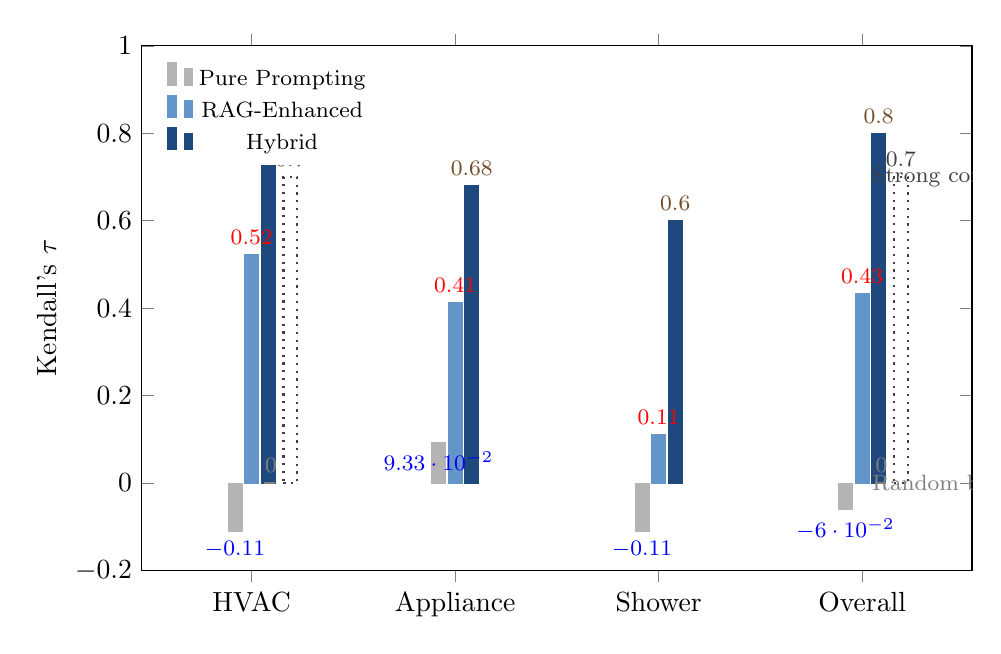
\begin{tikzpicture}
\begin{axis}[
	ybar,
	bar width=5pt,
	width=\columnwidth,
	height=0.68\columnwidth,
	symbolic x coords={HVAC,Appliance,Shower,Overall},
	xtick=data,
	ymin=-0.20,
	ymax=1.00,
	ytick={-0.2,0,0.2,0.4,0.6,0.8,1.0},
	ylabel={Kendall's $\tau$},
	enlarge x limits=0.18,
	legend style={at={(0.02,0.98)}, anchor=north west, font=\footnotesize, draw=none},
	nodes near coords={\pgfmathprintnumber[fixed,precision=2]{\pgfplotspointmeta}},
	point meta=y,
	every node near coord/.append style={font=\footnotesize}
]
\addplot+[
	draw=colorPure, fill=colorPure, bar shift=-6pt,
	nodes near coords,
	every node near coord/.append style={
		font=\footnotesize,
		anchor=north
	}
] coordinates {
	(HVAC,-0.1111) (Appliance,0.0933) (Shower,-0.1111) (Overall,-0.0600)
};
\addlegendentry{Pure Prompting}

\addplot+[draw=colorRAG, fill=colorRAG, bar shift=0pt, nodes near coords, every node near coord/.append style={anchor=south}] coordinates {
	(HVAC,0.5222) (Appliance,0.4133) (Shower,0.1111) (Overall,0.4333)
};
\addlegendentry{RAG-Enhanced}

\addplot+[draw=colorHybrid, fill=colorHybrid, bar shift=6pt, nodes near coords, every node near coord/.append style={anchor=south}] coordinates {
	(HVAC,0.9000) (Appliance,0.6800) (Shower,0.6000) (Overall,0.8000)
};
\addlegendentry{Hybrid}

\addplot[gray, dashed, thick] coordinates {(HVAC,0.00) (Overall,0.00)} node[pos=1, anchor=west, font=\footnotesize]{Random baseline};
\addplot[darkgray, dotted, thick] coordinates {(HVAC,0.70) (Overall,0.70)} node[pos=1, anchor=west, font=\footnotesize]{Strong correlation};
\end{axis}
\end{tikzpicture}
\caption{Kendall's $\tau$ by decision type and architecture. Dashed: $\tau=0$ (random). Dotted: $\tau=0.7$ (strong threshold).}
\label{fig:item10}
\end{figure}

%% =====================================================================
%% ITEM 11 -- Grouped Bar Chart: MAE per Criterion
%% =====================================================================
\begin{figure}[t]
\centering
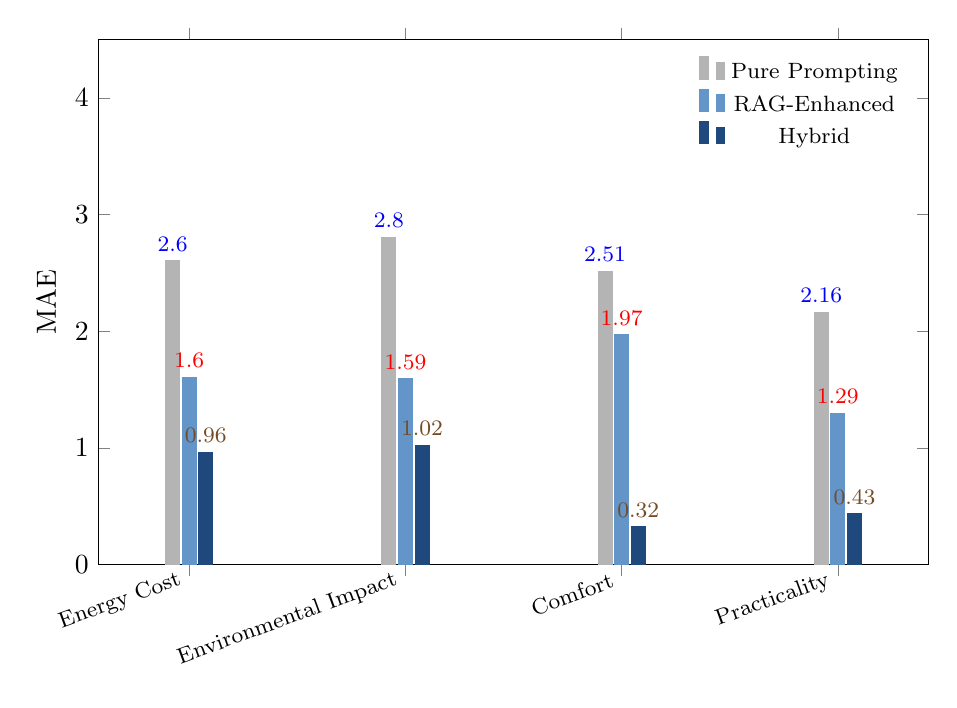
\begin{tikzpicture}
\begin{axis}[
	ybar,
	bar width=5pt,
	width=\columnwidth,
	height=0.68\columnwidth,
	symbolic x coords={Energy Cost,Environmental Impact,Comfort,Practicality},
	xtick=data,
	xticklabel style={font=\footnotesize, rotate=20, anchor=east},
	ymin=0,
	ymax=4.5,
	ylabel={MAE},
	enlarge x limits=0.14,
	legend style={at={(0.98,0.98)}, anchor=north east, font=\footnotesize, draw=none},
	nodes near coords={\pgfmathprintnumber[fixed,precision=2]{\pgfplotspointmeta}},
	point meta=y,
	every node near coord/.append style={font=\footnotesize, anchor=south}
]
\addplot+[draw=colorPure, fill=colorPure, bar shift=-6pt] coordinates {
	(Energy Cost,2.6037) (Environmental Impact,2.8042) (Comfort,2.5146) (Practicality,2.1619)
};
\addlegendentry{Pure Prompting}

\addplot+[draw=colorRAG, fill=colorRAG, bar shift=0pt] coordinates {
	(Energy Cost,1.6043) (Environmental Impact,1.5912) (Comfort,1.9696) (Practicality,1.2945)
};
\addlegendentry{RAG-Enhanced}

\addplot+[draw=colorHybrid, fill=colorHybrid, bar shift=6pt] coordinates {
	(Energy Cost,0.9622) (Environmental Impact,1.0238) (Comfort,0.3226) (Practicality,0.4332)
};
\addlegendentry{Hybrid}
\end{axis}
\end{tikzpicture}
\caption{MAE per criterion by architecture (Overall, $n=100$, scale 0--10).}
\label{fig:item11}
\end{figure}

%% =====================================================================
%% ITEM 12 -- Token and Latency Dual-Axis Figure
%% =====================================================================
\begin{figure}[t]
\centering
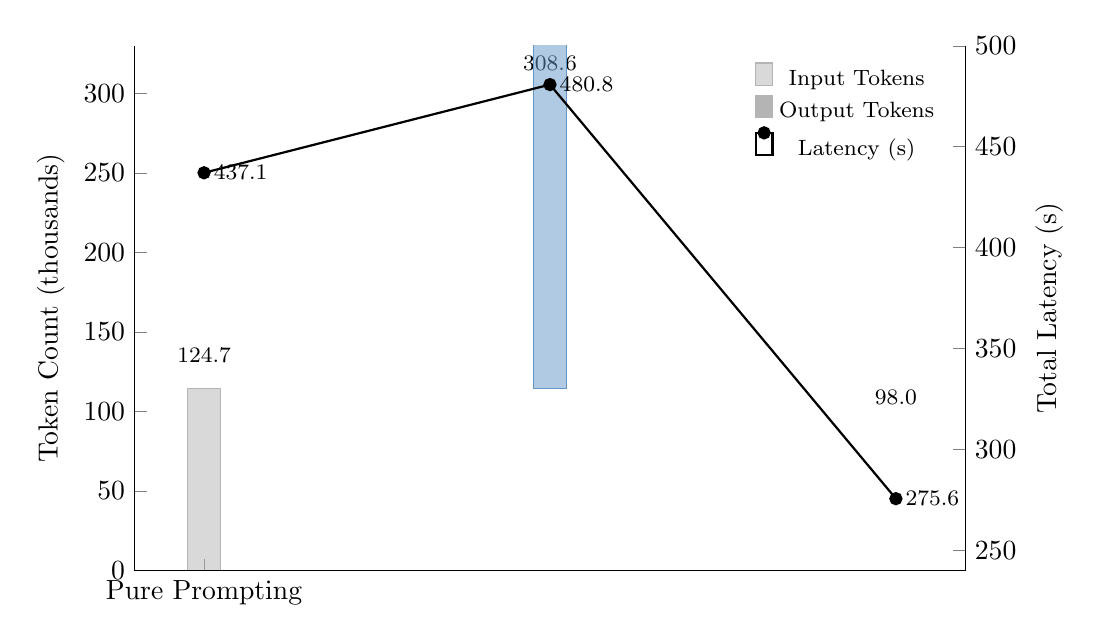
\begin{tikzpicture}
\begin{axis}[
	width=\columnwidth,
	height=0.68\columnwidth,
	axis y line*=left,
	axis x line*=bottom,
	ybar stacked,
	bar width=12pt,
	symbolic x coords={Pure Prompting,RAG-Enhanced,Hybrid},
	xtick=data,
	ymin=0,
	ymax=330,
	ylabel={Token Count (thousands)},
	legend style={at={(0.98,0.98)}, anchor=north east, font=\footnotesize, draw=none}
]
\addplot+[draw=colorPure, fill=colorPure, fill opacity=0.5] coordinates {(Pure Prompting,114.739)};
\addlegendentry{Input Tokens}
\addplot+[draw=colorRAG, fill=colorRAG, fill opacity=0.5, forget plot] coordinates {(RAG-Enhanced,295.174)};
\addplot+[draw=colorHybrid, fill=colorHybrid, fill opacity=0.5, forget plot] coordinates {(Hybrid,81.741)};

\addplot+[draw=colorPure, fill=colorPure] coordinates {(Pure Prompting,9.970)};
\addlegendentry{Output Tokens}
\addplot+[draw=colorRAG, fill=colorRAG, forget plot] coordinates {(RAG-Enhanced,13.463)};
\addplot+[draw=colorHybrid, fill=colorHybrid, forget plot] coordinates {(Hybrid,16.275)};
\addlegendimage{black, thick, mark=*, mark options={fill=black}}
\addlegendentry{Latency (s)}

\node[font=\footnotesize, anchor=south] at (axis cs:Pure Prompting,124.709) {124.7};
\node[font=\footnotesize, anchor=south] at (axis cs:RAG-Enhanced,308.637) {308.6};
\node[font=\footnotesize, anchor=south] at (axis cs:Hybrid,98.016) {98.0};
\end{axis}

\begin{axis}[
	width=\columnwidth,
	height=0.68\columnwidth,
	axis y line*=right,
	axis x line*=none,
	symbolic x coords={Pure Prompting,RAG-Enhanced,Hybrid},
	xtick=data,
	ymin=240,
	ymax=500,
	ylabel={Total Latency (s)},
	xtick=\empty
]
\addplot+[black, thick, mark=*, mark options={fill=black}] coordinates {
	(Pure Prompting,437.08342933654785)
	(RAG-Enhanced,480.7858417034149)
	(Hybrid,275.5911343097687)
};
\node[font=\footnotesize, anchor=west] at (axis cs:Pure Prompting,437.08342933654785) {437.1};
\node[font=\footnotesize, anchor=west] at (axis cs:RAG-Enhanced,480.7858417034149) {480.8};
\node[font=\footnotesize, anchor=west] at (axis cs:Hybrid,275.5911343097687) {275.6};
\end{axis}
\end{tikzpicture}
\caption{Token usage (stacked bars, left axis) and latency (line, right axis) per architecture across 100 scenarios.}
\label{fig:item12}
\end{figure}

%% =====================================================================
%% ITEM 13 -- Accuracy-Efficiency Tradeoff Scatter
%% =====================================================================
\begin{figure}[t]
\centering
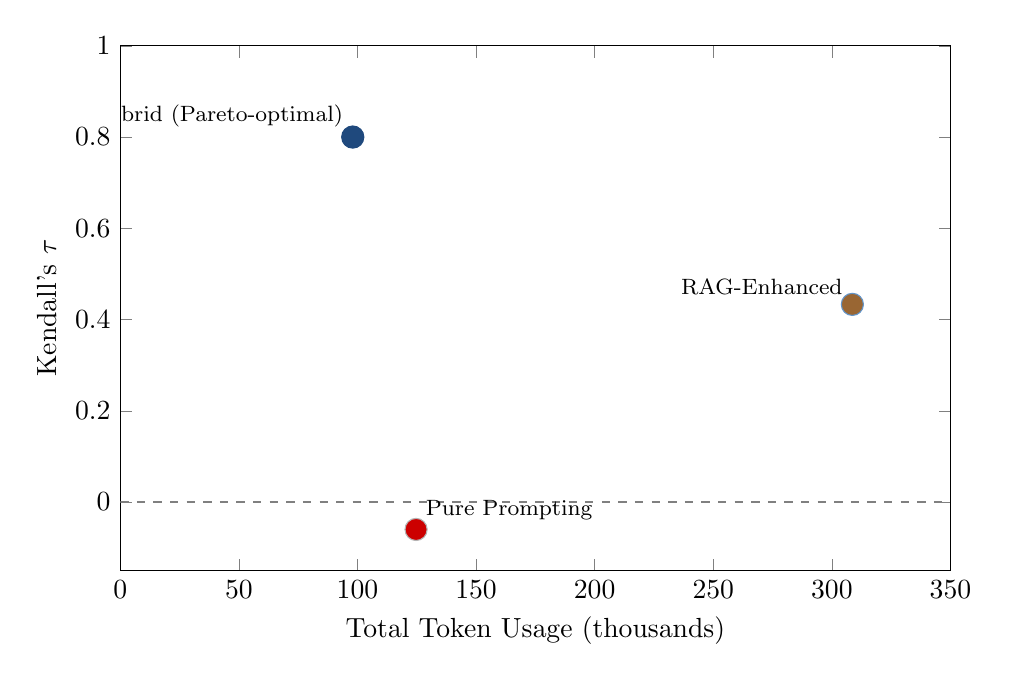
\begin{tikzpicture}
\begin{axis}[
	width=\columnwidth,
	height=0.68\columnwidth,
	xmin=0,
	xmax=350,
	ymin=-0.15,
	ymax=1.00,
	xlabel={Total Token Usage (thousands)},
	ylabel={Kendall's $\tau$}
]
\addplot[gray, dashed, thick] coordinates {(0,0) (350,0)} node[pos=1, anchor=west, font=\footnotesize]{Random baseline};

\addplot+[only marks, mark=*, mark size=4pt, draw=colorPure, fill=colorPure] coordinates {(124.709,-0.0600)};
\node[font=\footnotesize, anchor=south west] at (axis cs:124.709,-0.0600) {Pure Prompting};

\addplot+[only marks, mark=*, mark size=4pt, draw=colorRAG, fill=colorRAG] coordinates {(308.637,0.4333)};
\node[font=\footnotesize, anchor=south east] at (axis cs:308.637,0.4333) {RAG-Enhanced};

\addplot+[only marks, mark=*, mark size=4pt, draw=colorHybrid, fill=colorHybrid] coordinates {(98.016,0.8000)};
\node[font=\footnotesize, anchor=south east] at (axis cs:98.016,0.8000) {Hybrid (Pareto-optimal)};
\end{axis}
\end{tikzpicture}
\caption{Accuracy--efficiency tradeoff. Hybrid is Pareto-dominant: highest $\tau$ at lowest token cost.}
\label{fig:item13}
\end{figure}

%% =====================================================================
%% ITEM 14 -- Architecture Pipeline Diagram Placeholder
%% =====================================================================
\begin{figure*}[t]
\centering
\missingfigure[figwidth=\textwidth]{Side-by-side vertical pipeline flowcharts for three LLM integration architectures. Pure Prompting: 3 LLM calls, one per alternative, no external context. RAG-Enhanced: 3 LLM calls each preceded by ChromaDB retrieval (k=3 chunks). Hybrid: 1 LLM call for parameter extraction, output to physics-based calculator, then MAVT weighted sum.}
\caption{Processing pipeline for each architecture. Pure Prompting and RAG-Enhanced require three API calls per scenario; Hybrid requires one.}
\label{fig:pipeline}
\end{figure*}

\end{document}